\documentclass[conference, compsoc]{IEEEtran}
\usepackage{graphicx}
\usepackage{listings}
\usepackage{array, float}
\usepackage[colorlinks=true]{hyperref}
\usepackage[style=numeric,backend=bibtex]{biblatex}
\graphicspath{ {./figures/} }
\addbibresource{refs.bib}

\lstdefinestyle{model_arch}{
	backgroundcolor=\color{white},   
	basicstyle=\ttfamily,
	breaklines=true,
	showstringspaces=false,
	frame=single, % This adds a box around all sides of the snippet
	rulecolor=\color{black}, % You can specify the color of the box
}

\begin{document}
	\title{Dataset Distillation: A Data-Efficient Learning Framework}
	\author{Swapnil Patel - 999728870 - \today}
	
	\author{\IEEEauthorblockN{Swapnil Patel}
		\IEEEauthorblockA{
			University of Toronto\\
			swap.patel@mail.utoronto.ca\\
			Code: \href{https://github.com/Swapnil949/ECE1512\_2024F\_ProjectRepo\_SwapnilPatel}{Swapnil949/ECE1512\_2024F\_ProjectRepo\_SwapnilPatel}
	}}
	
	\maketitle
	
	\begin{abstract}
	\label{sec:abstract}
	This report explores dataset distillation techniques, focusing on the comparison between DataDAM and PAD methods for synthesizing compact datasets. Dataset distillation aims to generate smaller, synthetic datasets that retain essential information, enabling efficient training with reduced computational resources. Using the MNIST dataset as a benchmark, this study compares synthetic dataset generation using DataDAM’s Attention Matching and PAD’s alignment-focused approach. PAD’s methodology is implemented with modifications to support MNIST and incorporates a data selection strategy inspired by DeepCore. Additionally, DataDAM is applied to a larger dataset, MHIST, to evaluate its performance on more complex data.
	\end{abstract}
	
	\section{Introduction}
	\label{sec:intro}
	
	Dataset Distillation is an emerging technique in machine learning designed to compress large datasets into smaller, synthetic datasets that retain the critical information needed to train neural networks effectively. This approach addresses the growing demand for computational efficiency by significantly reducing memory requirements and training times without compromising model performance. By distilling the essential features of a vast dataset, researchers can train models on a compact, representative subset, thus enabling rapid prototyping and exploration of deep learning architectures. As dataset sizes continue to expand, methods such as dataset distillation offer promising pathways for scalable and resource-efficient machine learning. 
	
	Dataset distillation has several applications such as \textit{Neural Architecture Search (NAS)}, \textit{Privacy Preservation}, \textit{Federated Learning}, \textit{Memory-efficient Continual Learning}, and \textit{Data sharing}.
	
	\subsubsection*{Neural Architecture Search (NAS)}
	In NAS, dataset distillation provides a compact proxy dataset that approximates the performance of training on a full-scale dataset \cite{white2023neuralarchitecturesearchinsights}. This enables faster and more resource-efficient model evaluation across architectures, allowing for rapid exploration and selection of optimal models without the computational expense of using the full dataset.
	
	\subsubsection*{Privacy Preservation}
	For privacy preservation, distilled datasets reduce exposure to sensitive information by retaining only essential features rather than raw, identifiable data \cite{dong2022privacyfreedoesdataset}. This allows machine learning models to be trained securely in privacy-sensitive domains (e.g., healthcare and finance) and enhances data sharing compliance in settings like federated learning.
	
	All experiments and results in this report were conducted using the following setup: \hfill
	
	\begin{itemize}
		\item \texttt{\textbf{CPU:} AMD EPYC 7B13}
		\item \texttt{\textbf{PyTorch ver.:} 2.2.1}
		\item \texttt{\textbf{GPU:} NVIDIA GeForce RTX 4090}
		\item \texttt{\textbf{CUDA ver:} 8.9}
		\item \texttt{\textbf{Total Memory:} 23.65 GB}
	\end{itemize}	
	
	\section{Dataset Distillation with Attention Matching}
	The paper "DataDAM: Efficient Dataset Distillation with Attention Matching" \cite{sajedi2023datadamefficientdatasetdistillation} presents a novel dataset distillation approach aimed at reducing training dataset sizes while retaining essential information. The primary challenge addressed by the authors is the high computational cost associated with deep learning models when using full-sized datasets.
	
	In this work, the authors generate a synthetic dataset by employing \texttt{Spatial Attention Mapping (SAM)} to capture attention maps from real and synthetic data across various layers within a family of randomly initialized neural networks. This approach alleviates the substantial memory demands typically encountered in state-of-the-art methods. The use of randomly initialized neural network instead of Pre-trained models also makes their solution more versatile and improves cross-architecture generalization results. 
	
	Additionally, they introduce a \texttt{complementary loss} as a regularization technique to align the last-layer feature distributions between the real and synthetic datasets. Fig. \ref{fig:datadam_method} illustrates the novel methodology proposed by the authors.
	
	% Privacy 
	
	% neural Network search
	
	\begin{figure}[H]
		\centering
		\includegraphics[width=0.48\textwidth]{datadam.png}
		\caption{DataDAM Method \cite{sajedi2023datadamefficientdatasetdistillation}}
		\label{fig:datadam_method}
	\end{figure}
	
	With this new method, authors are able to beat existing state-of-the-art solutions by improving performance by 6.5\% for CIFAR100 and 4.1\% for ImageNet-1k. They also achieve up to a 100x reduction in training costs for learning synthetic dataset.
	
	\subsection{MNIST Dataset}
	\begin{figure}[H]
		\centering
		\includegraphics[width=0.48\textwidth]{MNIST_dataset.png}
		\caption{MNIST Dataset \cite{deng2012mnist}}
		\label{fig:mnist_dataset}
	\end{figure}
	The MNIST dataset is a widely used collection of handwritten digits that is commonly used for training and testing machine learning and computer vision algorithms. MNIST stands for the "Modified National Institute of Standards and Technology" database. It was created by modifying the original NIST dataset, which contained a much larger and more diverse set of handwritten characters, to focus specifically on handwritten digits.
	
	The MNIST dataset contains 28x28-pixel grayscale images of handwritten digits (0 through 9), along with corresponding labels indicating which digit each image represents \cite{deng2012mnist}. There are 60,000 training images and 10,000 testing images in the MNIST dataset, making it a popular benchmark for various image classification tasks.
	
	\subsubsection{ConvNet-3} \hfill
	
	A ConvNet-3 model was trained using the original MNIST data, utilizing Stochastic Gradient Descent (SGD) as the optimizer. The training process incorporated a cosine annealing scheduler with a learning rate of 0.01 over 20 epochs. The training and test accuracy are presented below in Figure \ref{fig:ConvNet3_training_testing_accuracy}.
	
	\begin{figure}[H]
		\centering
		\includegraphics[width=0.48\textwidth]{ConvNet3_training_testing_accuracy.png}
		\caption{MNIST Dataset Accuracy with ConvNet-3 Model with Original dataset}
		\label{fig:ConvNet3_training_testing_accuracy}
	\end{figure}
	
	Table \ref{tab:convet3_results} summarizes the training time to Train the ConvNet3 model with oriignal MNIST dataset as well as total FLOPS.    
	\begin{table}[H]
		\caption{ConvNet3 with Original MNIST}
		\centering
		\label{tab:convet3_results}
		\begin{tabular}{|c|c|}
			\hline
			Training Time & 255.49 s\\
			\hline
			FLOPS & 48,429,056 \\
			\hline
		\end{tabular}
	\end{table}
	
	\subsubsection{Synthetic Dataset using real images} \hfill
	
	A codebase from DataDAM \cite{sajedi2023datadamefficientdatasetdistillation} paper was adapted to implement the Attention Matching algorithm for learning the synthetic dataset. The resulting code can be found in the project repository, linked above.
	
	
	A synthetic dataset $\mathcal{S}$ was created by randomly selecting 10 images per class from the original dataset. These images served as the starting point for the initialization of condensed images in the Attention Matching algorithm \cite{sajedi2023datadamefficientdatasetdistillation}, which was then applied to learn the synthetic dataset $\mathcal{S}$. The experimental setup, including the hyper-parameters $K$, $T$, $\eta_S$, $\zeta_S$, $\eta_{\theta}$, and $\zeta_{\theta}$, is outlined below in table \ref{table:parameters_mnist}.
	
	\begin{table}[H]
		\centering	
		\caption{Hyper-parameters for learning $\mathcal{S}$ from MNIST dataset}
		\begin{tabular}{|c|c|}
			\hline
			\textbf{Parameter} & \textbf{Value} \\ \hline
			K & 100 \\ \hline
			T & 10 \\ \hline
			$\eta$ & 0.1 \\ \hline
			$\zeta_S$ & 1 \\ \hline
			$\eta_{\theta}$ & 0.01 \\ \hline
			$\zeta_{\theta}$ & 50 \\ \hline
			Optimizer & SGD \\ \hline
			\# images/class & 10 \\ \hline
			Minibatch size & 256 \\ \hline
		\end{tabular}
		\label{table:parameters_mnist}
	\end{table}
	
	
	In Figure~\ref{fig:mnist_real_sample}, one sample from each class, chosen to initialize the synthetic dataset $\mathcal{S}$, is shown. In Figure~\ref{fig:mnist_real_syn}, the transformation of these images is illustrated, showing how each sample appears after the dataset condensation process has been completed.
	\begin{figure}[H]
		\centering
		\includegraphics[width=0.48\textwidth]{mnist_real_sample.png}
		\caption{Sample of Synthetic MNIST Dataset created from real images (starting image)}
		\label{fig:mnist_real_sample}
	\end{figure}
	
	\begin{figure}[H]
		\centering
		\includegraphics[width=0.48\textwidth]{mnist_real_syn.png}
		\caption{Sample of Synthetic MNIST Dataset created from real images (final image)}
		\label{fig:mnist_real_syn}
	\end{figure}
	
	As illustrated, the condensed image resembles a blend of multiple data samples, characterized by the presence of blurred digits. Despite this blurriness, the resultant condensed images remain discernible, allowing digits to be easily identified by the human eye; however, they are not as clear as the original images.
	
	In Figure \ref{fig:mnist_real_syn_all}, the entire learned synthetic dataset $\mathcal{S}$ is presented, showcasing 10 synthetic images per class that have been generated through the condensation process using attention matching algorithm \cite{sajedi2023datadamefficientdatasetdistillation}.
	
	\begin{figure}[H]
		\centering
		\includegraphics[width=0.48\textwidth]{mnist_real_syn_all.png}
		\caption{Synthetic MNIST Dataset created from real images}
		\label{fig:mnist_real_syn_all}
	\end{figure}
	\subsubsection{Synthetic Dataset using Gaussian noise} \hfill
	
	Similarly, the synthetic dataset was learned using random Gaussian noise as the initial images. This approach provides several benefits, including robustness to overfitting, as the model is encouraged to generalize rather than memorize specific patterns from the training data. By exploring the feature space with diverse noise variations, the model can uncover latent representations that may not be evident with structured initial images. Additionally, using Gaussian noise simplifies the initialization process, allowing for faster setup without the need for selecting specific samples from the original dataset. Overall, this method can potentially enhances the model's ability to learn robust and diverse representations, ultimately improving its performance over using real dataset.
	
	In Figure \ref{fig:mnist_noise_sample} below, the initial samples consisting of random Gaussian noise are shown. Figure \ref{fig:mnist_noise_syn}	 displays the resultant condensed images generated from these initial samples.
	
	\begin{figure}[H]
		\centering
		\includegraphics[width=0.48\textwidth]{mnist_noise_sample.png}
		\caption{Sample of Synthetic MNIST Dataset created from Gaussian noise (starting image)}
		\label{fig:mnist_noise_sample}
	\end{figure}
	
	\begin{figure}[H]
		\centering
		\includegraphics[width=0.48\textwidth]{mnist_noise_syn.png}
		\caption{Sample of Synthetic MNIST Dataset created from Gaussian noise (final image)}
		\label{fig:mnist_noise_syn}
	\end{figure}
	
	As shown in the figure \ref{fig:mnist_noise_syn_all}, the digits are not as easily identifiable by the human eye compared to the condensed images learned from real images. However, some digits, such as 0 and 1, remain recognizable, indicating that the synthetic dataset learning process was successful.
	
	\begin{figure}[H]
		\centering
		\includegraphics[width=0.48\textwidth]{mnist_noise_syn_all.png}
		\caption{Synthetic MNIST Dataset created from Gaussian noise}
		\label{fig:mnist_noise_syn_all}
	\end{figure}
	
	In Figure \ref{fig:mnist_noise_syn_all}, the complete learned synthetic dataset $\mathcal{S}$ is displayed, featuring 10 synthetic images per class that have been generated through the condensation process using random Gaussian noise as the initial input.
	
	The comparison between synthetic datasets learned from real images and those initialized with Gaussian noise highligHs significant differences in both quality and performance. The dataset derived from real images results in clearer, more recognizable digits, allowing for effective learning and higher accuracy rates. In contrast, the dataset initialized with Gaussian noise exhibits a lack of clarity, with many digits becoming ambiguous and overall performance metrics declining. However, it is important to note that starting from Gaussian noise can potentially yield a more generalized synthetic dataset, although it may require significantly more iterations to achieve comparable results. Both approaches have their pros and cons, and depending on the specific application, each method has its place in the dataset condensation process.
	
	\subsubsection{ConvNet-3 using Synthetic Dataset} \hfill
	
	This section examines the performance of the ConvNet-3 model when trained on a synthetic dataset generated through the dataset distillation process discussed earlier. The synthetic dataset comprises 100 training images, in contrast to the full MNIST dataset used in the previous experiment. The same training setup that was used to train ConvNet-3 for the entire MNIST dataset was also employed here, including the use of Stochastic Gradient Descent (SGD) as the optimizer and a cosine annealing scheduler with a learning rate of 0.01 over 20 epochs.
	\begin{figure}[H]
		\centering
		\includegraphics[width=0.48\textwidth]{mnist_syn_acc.png}
		\caption{ConvNet-3 Model Trained using Original and Synthetic dataset}
		\label{fig:mnist_syn_acc}
	\end{figure}
	Figure \ref{fig:mnist_syn_acc} shows the results of the training and test accuracy of the ConvNet-3 model when trained with both the original and synthetic datasets. This comparison highligHs the performance differences between using the full MNIST dataset and the distilled synthetic dataset. As can be seen, the training accuracy for the synthetic dataset is almost the same as the training accuracy for the original dataset after 20 epochs. While, the test accuracy for the synthetic dataset is approximately 0.8 after 20 epochs, which is lower than the test accuracy achieved with the original dataset
	\begin{figure}[H]
		\centering
		\includegraphics[width=0.48\textwidth]{mnist_syn_time.png}
		\caption{ConvNet-3 Model Training time for Original and Synthetic dataset}
		\label{fig:mnist_syn_time}
	\end{figure}
	Figure \ref{fig:mnist_syn_time} compares the training time for the ConvNet-3 model using the original and synthetic datasets. This is where the advantages of using the synthetic dataset become clear: the original dataset took approximately 255 seconds to train, while the synthetic dataset only took 32 seconds to train, which is an 87.5\% reduction in training time.
	\subsubsection{Cross-architecture Generalization - AlexNet}\hfill
	
	In dataset distillation, cross-architecture generalization is crucial for ensuring that synthetic datasets are versatile and can effectively transfer learned features across diverse model architectures, enhancing their robustness and applicability in real-world scenarios. To demonstrate this capability, an AlexNet model was trained using the synthetic dataset.
	
	\begin{figure}[H]
		\centering
		\includegraphics[width=0.48\textwidth]{mnist_alex_acc.png}
		\caption{AlexNet Model Trained using Synthetic dataset}
		\label{fig:mnist_alex_acc}
	\end{figure}
	
	AlexNet was trained on the synthetic dataset using the following parameters: 100 epochs, a learning rate of 0.01, and cross-entropy loss as the criterion, optimized with SGD. Figure \ref{fig:mnist_alex_acc} illustrates the training and test accuracy for the AlexNet model. As shown, after approximately 80 epochs, the test accuracy stabilizes around 0.8—matching the accuracy achieved by the ConvNet model—demonstrating successful cross-architecture generalization.
	
	\subsection{MHIST Dataset}
	The MHIST dataset, short for "Minimalist Histopathology Image Screening Test," is a specialized dataset commonly used for training and evaluating machine learning models in the field of digital pathology. It was developed to address specific challenges in histopathological image analysis, focusing particularly on the differentiation between types of colorectal polyp tissues.
	
	The MHIST dataset contains 224x224-pixel RGB images of hematoxylin and eosin (H\&E) stained histopathology slides, with labels distinguishing between two classes: Hyperplastic Polyp (non-cancerous) and Sessile Serrated Adenoma Polyp (pre-cancerous). It consists of 3,152 image patches divided into 2,456 training images and 696 testing images, making it a valuable resource for binary classification tasks in medical image analysis \cite{wei2021petri}.
	\begin{figure}[H]
		\centering
		\includegraphics[width=0.48\textwidth]{MHIST_dataset.png}
		\caption{MHIST Dataset \cite{wei2021petri}}
		\label{fig:mhist_dataset}
	\end{figure}
	\subsubsection{ConvNet-7} \hfill
	
	A ConvNet-7 model was trained on MHIST dataset, using SGD with cosine annealing and a learning rate of 0.01 over 20 epochs. Figure \ref{fig:mhist_convnet7_acc} shows the resulting accuracy for training and testing datasets.
	\begin{figure}[H]
		\centering
		\includegraphics[width=0.48\textwidth]{mhist_convnet7_acc.png}
		\caption{MHIST Dataset Accuracy with ConvNet-7 Model with Original dataset}
		\label{fig:mhist_convnet7_acc}
	\end{figure}
	
	\begin{table}[H]
		\caption{ConvNet7 with Original MHIST}
		\centering
		\label{tab:convet7_results}
		\begin{tabular}{|c|c|}
			\hline
			Training Time & 466.05 s\\
			\hline
			FLOPS & 2,640,717,952 \\
			\hline
		\end{tabular}
	\end{table}
	
	\subsubsection{Synthetic Dataset using real images} \hfill
	
	Similar to MNIST dataset, a synthetic dataset $\mathcal{S}$ was learned by randomly selecting 50 images per classs from the original dataset. The experimental setup, iincluding the hyper-parameters $K$, $T$, $\eta_S$, $\zeta_S$, $\eta_{\theta}$, and $\zeta_{\theta}$, used to learn this syntehtic dataset is outlined below in table \ref{table:parameters_mhist}.
	
	The parameter $\zeta_S$ was adjusted from the recommended value of $0.1$ to $5.0$ following the guidelines of the Attention Matching Algorithm \cite{sajedi2023datadamefficientdatasetdistillation}. An additional experiment with $\zeta_S$ set to $0.1$ was conducted, but this setting required substantially longer iterations to yield a meaningful synthetic dataset.
	
	\begin{table}[H]
	\centering
	\caption{Hyper-parameters for learning $\mathcal{S}$ from MHIST dataset}
	\begin{tabular}{|c|c|}
		\hline
		\textbf{Parameter} & \textbf{Value} \\ \hline
		K & 200 \\ \hline
		T & 10 \\ \hline
		$\eta$ & 5.0 \\ \hline
		$\zeta_S$ & 1 \\ \hline
		$\eta_{\theta}$ & 0.01 \\ \hline
		$\zeta_{\theta}$ & 50 \\ \hline
		Optimizer & SGD \\ \hline
		\# images/class & 50 \\ \hline
		Minibatch size & 128 \\ \hline
	\end{tabular}
	\label{table:parameters_mhist}
	\end{table}	

	
	\begin{figure}[H]
		\centering
		\includegraphics[width=0.48\textwidth]{mhist_real_sample.png}
		\caption{Sample of Synthetic MHIST Dataset created from real images (starting image)}
		\label{fig:mhist_real_sample}
	\end{figure}
	\begin{figure}[H]
		\centering
		\includegraphics[width=0.48\textwidth]{mhist_real_syn.png}
		\caption{Sample of Synthetic MHIST Dataset created from real images (final image)}
		\label{fig:mhist_real_final}
	\end{figure}
	
	Figure \ref{fig:mhist_real_sample} displays one sample from each class of the selected images before dataset condensation. Figure \ref{fig:mhist_real_final} illustrates the transformation of these samples after the condensation process is complete.
	
	As seen in the original images, HP and SSA classes are easily distinguishable. However, in the condensed images, distinguishing features are nearly unrecognizable, with several new abstract features added during the condensation process.
	
	Figure \ref{fig:mhist_real_syn_hp} presents all 50 condensed images from the HP class, while Figure \ref{fig:mhist_real_syn_ssa} shows the corresponding set for the SSA class.
	
	\vfill
	\begin{figure}[H]
		\centering
		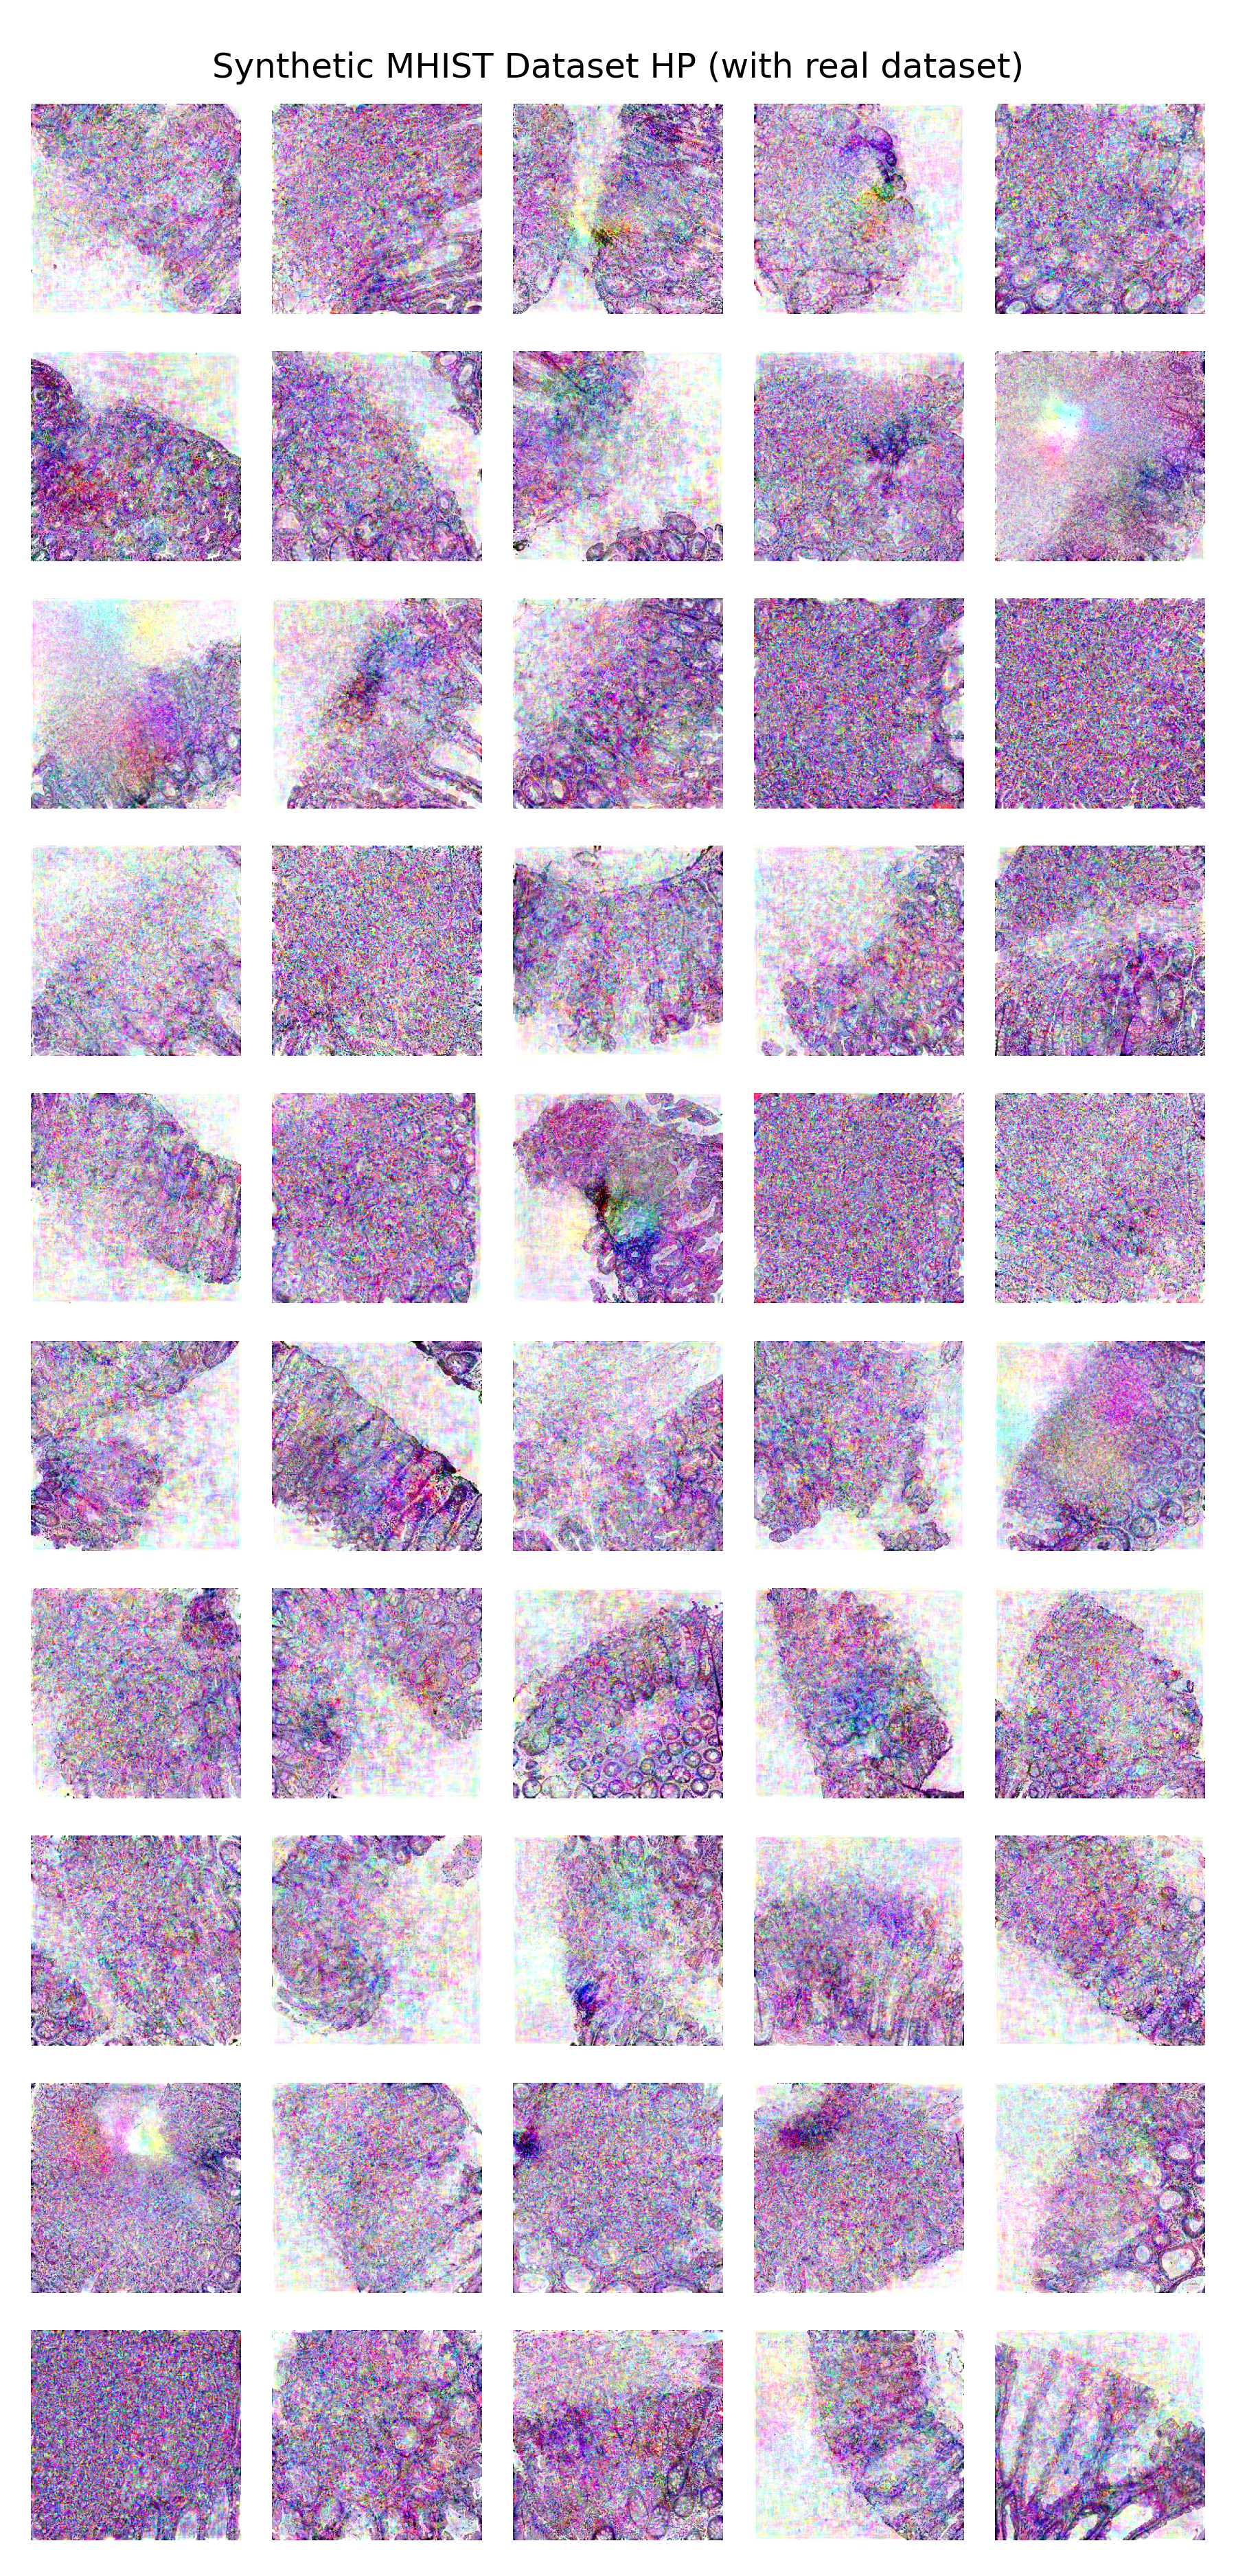
\includegraphics[width=0.48\textwidth]{mhist_real_syn_hp.png}
		\caption{Synthetic MHIST Dataset created from real images [HP]}
		\label{fig:mhist_real_syn_hp}
	\end{figure}
	
	\begin{figure}[H]
		\centering
		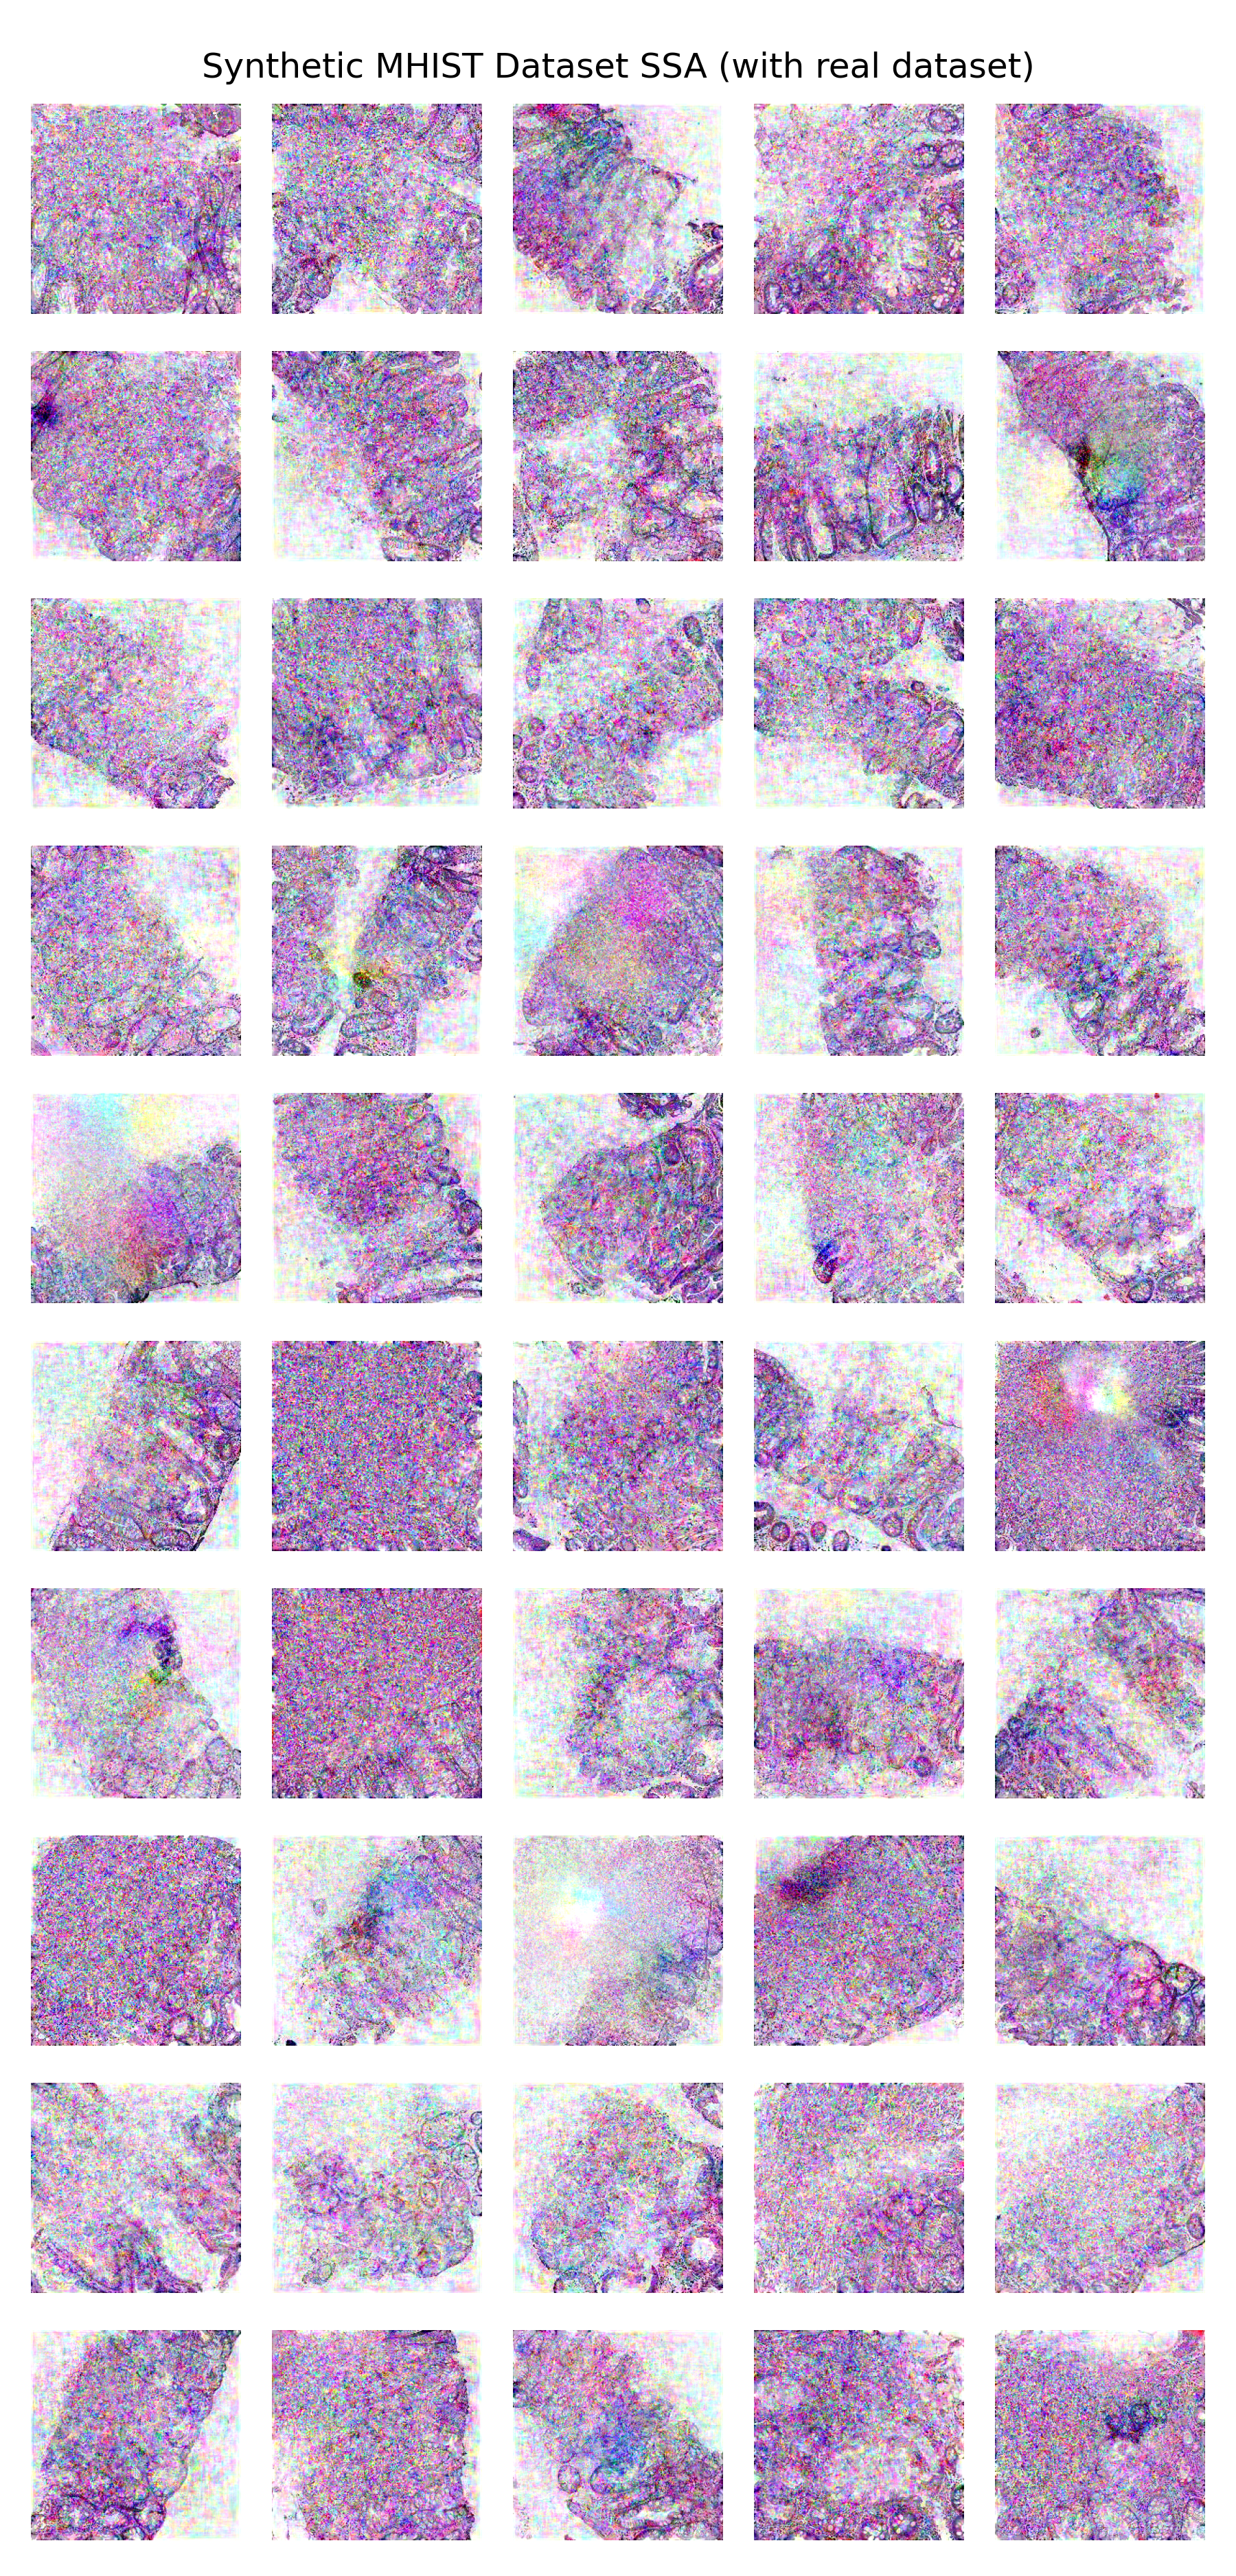
\includegraphics[width=0.48\textwidth]{mhist_real_syn_ssa.png}
		\caption{Synthetic MHIST Dataset created from real images [SSA]}
		\label{fig:mhist_real_syn_ssa}
	\end{figure}
	\vfill
	
	\subsubsection{Synthetic Dataset using Gaussian noise} \hfill
	
	Another synthetic dataset, $\mathcal{S}$, was generated using Gaussian noise as the initial images. Figure \ref{fig:mhist_noise_sample} shows the starting images, and Figure \ref{fig:mhist_noise_final} presents the corresponding condensed images. 
	
	\begin{figure}[H]
		\centering
		\includegraphics[width=0.48\textwidth]{mhist_noise_sample.png}
		\caption{Sample of Synthetic MHIST Dataset created from Gaussian noise (starting image)}
		\label{fig:mhist_noise_sample}
	\end{figure}
	\begin{figure}[H]
		\centering
		\includegraphics[width=0.48\textwidth]{mhist_noise_sample.png}
		\caption{Sample of Synthetic MHIST Dataset created from Gaussian noise(final image)}
		\label{fig:mhist_noise_final}
	\end{figure}
	
	Unlike the MNIST dataset, this synthetic dataset is barely recognizable. While MNIST images are grayscale and consist of simple digits, MHIST images are in RGB and contain abstract features, making the condensed images difficult for human interpretation. Running the attention algorithm for additional iterations or with a higher learning rate could have potentially improved the results for the Gaussian case. However, due to resource constraints, compute time was prioritized for synthetic datasets generated from real images.
	
	Figure \ref{fig:mhist_noise_syn_all} shows larger sample of synthetic MHIST dataset generated from Gaussian noise. Similar to sample shown in figures above, these images are also indistinguishable. 
	
	\begin{figure}[H]
		\centering
		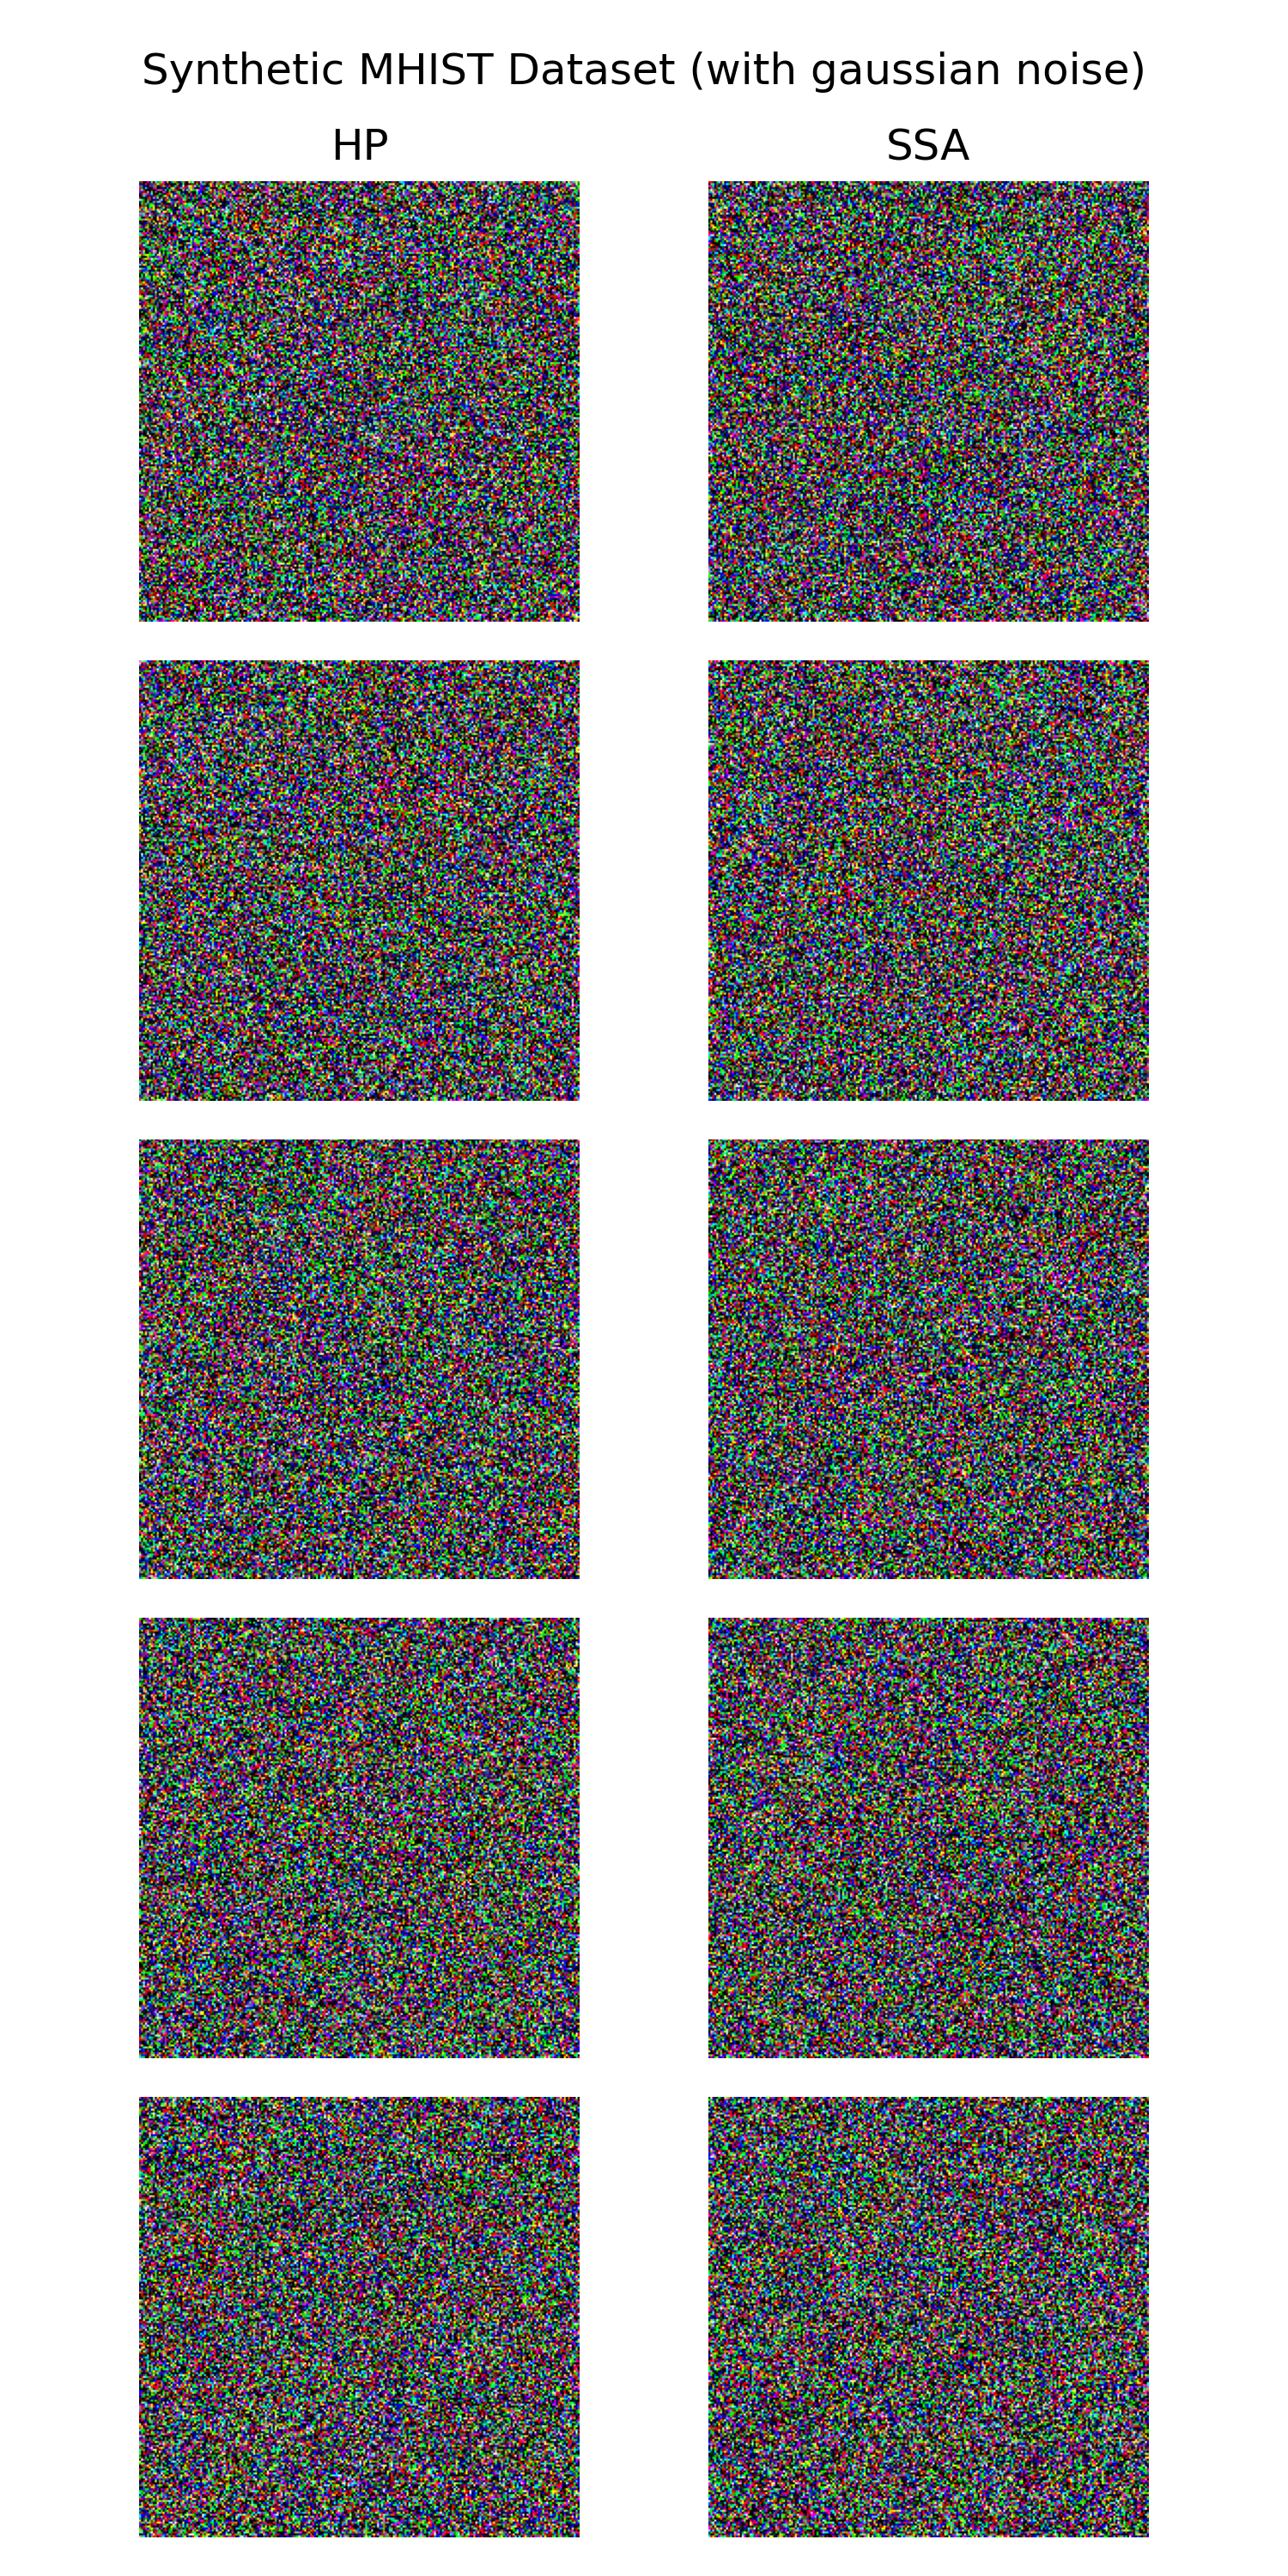
\includegraphics[width=0.48\textwidth]{mhist_noise_syn_all.png}
		\caption{Synthetic MHIST Dataset created from Gaussian noise}
		\label{fig:mhist_noise_syn_all}
	\end{figure}
	
	\subsubsection{ConvNet-7 using Synthetic Dataset} \hfill
	
	To validate the synthetic dataset, a ConvNet-7 model was trained on it and evaluated against the test set, following the same setup as described earlier. Figure \ref{fig:mhist_syn_acc} shows the training and test accuracies for ConvNet-7 models using both the original and synthetic datasets. Training accuracy for both datasets saturates at 1.0 after around 15 epochs. However, while the model trained on the original dataset achieves a test accuracy of approximately 0.75, indicating model limitations, the model trained on the synthetic dataset only reaches around 0.6, demonstrating a significant performance gap.
	
	\begin{figure}[H]
		\centering
		\includegraphics[width=0.48\textwidth]{mhist_syn_acc.png}
		\caption{ConvNet-7 Model Trained using Original and Synthetic dataset}
		\label{fig:mhist_syn_acc}
	\end{figure}
	
	The poor results with the condensed dataset may arise from several issues. The condensation process might have removed important details from the original images, leading to oversimplified representations. Additionally, if the synthetic dataset lacks diversity or does not fully capture class variability, the model may struggle to generalize. The complexity of the MHIST dataset, with its RGB images and abstract features, may also challenge ConvNet-7's performance, which might require different hyperparameters or longer training to improve results.
	
	However, as shown in Figure \ref{fig:mhist_syn_time}, there is still significant reduction in training time when using the smaller condensed dataset, aligning with our expectations.
	
	\begin{figure}[H]
		\centering
		\includegraphics[width=0.48\textwidth]{mhist_syn_time.png}
		\caption{ConvNet-7 Model Training time for Original and Synthetic dataset}
		\label{fig:mhist_syn_time}
	\end{figure}
	\subsubsection{Cross-architecture Generalization - ResNet-18} \hfill
	
	To test for cross-architecture generalization, the MHIST synthetic dataset was evaluated using the ResNet-18 model. The results shown in Figure \ref{fig:mhist_resnet_acc}, indicated poor performance in both training and test accuracy, which can be attributed to several factors. The complexity of the synthetic dataset may have overwhelmed the model's architecture, leading to difficulties in learning meaningful features. Additionally, improper hyperparameter selection and limited compute resources likely hindered the model's ability to converge effectively. The choice of network architecture may also not have been optimal for the characteristics of the synthetic data, further contributing to the observed limitations in performance.

	\begin{figure}[H]
		\centering
		\includegraphics[width=0.48\textwidth]{mhist_resnet_acc.png}
		\caption{ResNet-18 Model Trained using Synthetic dataset}
		\label{fig:mhist_resnet_acc}
	\end{figure}
	
	\subsection{Data Distillation Application}
	
	To demonstrate the usefulness of dataset distillation, one of the applications mentioned in the introduction, Neural Architecture Search (NAS) was employed to illustrate the advantages of using synthetic datasets over the entire dataset. This approach highlights how synthetic datasets can lead to improved model efficiency and performance, enabling more effective exploration of architecture configurations while reducing computational costs associated with training on larger datasets.
	
	Briefly, Neural Architecture Search (NAS) is utilized to automate the process of designing neural network architectures, allowing for the optimization of various configurations to improve performance on targeted tasks \cite{white2023neuralarchitecturesearchinsights}. In this case, NAS was specifically applied to the MNIST dataset.
	
	To illustrate this, a simple fully connected network was configured with various combinations of layer and neuron sizes. Each resulting architecture was trained using both the original and synthetic datasets, and the best-performing architectures from each dataset were then compared.
	
	The search process with the original dataset took \textbf{1607.3 seconds}, while the same search process using the synthetic dataset only required \textbf{2.8 seconds}. Notably, the best-performing architecture identified from both datasets was identical, demonstrating the effectiveness of Neural Architecture Search (NAS) in leveraging synthetic datasets for efficient model optimization.
	
	\begin{figure}[H]
		\centering
		\includegraphics[width=0.48\textwidth]{nas_comparision.png}
		\caption{NAS best model with original vs synthetic MNIST dataset}
		\label{fig:nas_comparision}
	\end{figure}

	For reference, Figure \ref{fig:nas_comparision} presents a comparison of the test accuracies for the model configured with the best architecture identified from both the original and synthetic datasets.
	\section{Prioritize Alignment in Dataset Distillation}
		The paper, "Prioritize Alignment in Dataset Distillation (PAD)" \cite{li2024prioritizealignmentdatasetdistillation}, proposes a novel dataset distillation approach that seeks to address the problem of misaligned information in the information extraction and embedding phases. Existing distillation methods compress large datasets into smaller synthetic datasets, but the authors observed that these methods often introduce noise from irrelevant data and shallow-layer information, which can degrade the quality of distilled datasets.
	
	The key contributions by authors are as follows:
	\begin{itemize}
		\item \textbf{Data Filtering:} PAD introduces a data pruning strategy in the Information Extraction phase, which selects samples based on their difficulty levels relative to the distillation compression ratio. Specifically, simpler samples are prioritized when the compression ratio is high, while more challenging samples are included in low-compression scenarios. This aligns the extracted information more closely with the synthetic dataset's requirements.
		\item \textbf{Parameter Filtering:} In the Information Embedding phase, PAD selectively masks shallow-layer parameters of the agent model to reduce redundant low-level signals, which are not essential for accurate dataset distillation. Instead, it focuses on deeper layers to capture high-level features that improve the synthetic dataset's performance across models and architectures
	\end{itemize}
	
	\textbf{Evaluation:} The PAD method, tested on benchmarks like CIFAR-10, CIFAR-100, and Tiny ImageNet, showed substantial improvements over prior distillation techniques, particularly in high-compression settings. Its efficacy was demonstrated with both trajectory matching and mainstream matching-based distillation algorithms.
	
	This combination of sample difficulty alignment and deep-layer filtering marks PAD as a significant advancement, achieving state-of-the-art results and enhancing the generalization capability of distilled datasets across different model architectures.
	
	However, the method's effectiveness may decline for extremely large datasets such as ImageNet \cite{5206848} if additional misalignment issues arise from complex, high-dimensional features beyond the scope of current alignment strategies.
	
	Overall, PAD can provide state-of-the-art solutions for small to medium-sized datasets or datasets with moderate compression ratios such as CIFAR-10 and CIFAR-100 \cite{Krizhevsky2009LearningML}, where alignment of sample difficulty and deep-layer features is critical for effective distillation. However, it may have some shortcomings for very large-scale datasets, such as ImageNet \cite{5206848}, or datasets requiring complex, high-dimensional feature capture, as PAD's data pruning and shallow-layer masking may not fully preserve the rich hierarchical information needed for such datasets.
	
	\subsection{Synthetic Dataset}
	
	The PAD methods were implemented on the MNIST dataset due to its smaller image size (28x28) and single grayscale channel, which require fewer computational resources. Additionally, DataDAM demonstrated more promising results on MNIST than on MHIST, making MNIST results a more suitable choice for comparing the performance of PAD against DataDAM.
	
	The implementation process began with adapting the reference code from the Prioritize Alignment in Dataset Distillation (PAD) \cite{li2024prioritizealignmentdatasetdistillation} paper. The original code did not support the MNIST dataset, which uses 28x28 grayscale images rather than RGB images typically handled by PAD. Therefore, the code was extended to include MNIST, with adjustments made to accommodate its specific input shape and grayscale format.
	
	In addition, PAD’s methodology depends on a data selection strategy, termed \texttt{sort\_method}, to rank and select samples based on their relevance to distillation quality. This component was not available for MNIST in the reference code. To generate this, code from DeepCore: A Comprehensive Library for Coreset Selection in Deep Learning \cite{guo2022deepcorecomprehensivelibrarycoreset} was utilized. DeepCore provides techniques for sample selection and prioritization, which are commonly applied in deep learning to create representative, compact datasets. By adapting these principles, a \texttt{sort\_method} was developed for MNIST, allowing PAD to effectively prioritize and select data samples within this dataset.
	
	The adapeted code for PAD along with the file for \texttt{sort\_method} for MNIST dataset can be found within \texttt{src/task2/PAD} directory of the project repository.
	
	Using methodlogy discussed above, a syntehtic dataset cosnsiting of 10 images per class from MNIST dataset was generated. The resulting synnthetic dataset is shown below in Figure \ref{fig:synthetic_images_task2}.
	
	\begin{figure}[H]
		\centering
		\includegraphics[width=0.48\textwidth]{synthetic_images_task2.png}
		\caption{Synthetic MNIST Dataset using PAD\cite{li2024prioritizealignmentdatasetdistillation}}
		\label{fig:synthetic_images_task2}
	\end{figure}
	Visually, this synthetic dataset appears nearly identical to the dataset generated by DataDAM shown in Figure \ref{fig:mnist_real_syn_all}. However, to objectively compare the quality of the synthetic datasets, a ConvNet-3 model was trained using this new synthetic dataset, following the same approach as in the previous section with the DataDAM-generated synthetic dataset.
	
	In Figure \ref{fig:train_acc_task2}, the training accuracy is compared across the original MNIST dataset, the synthetic dataset generated by DataDAM, and the synthetic dataset generated by PAD. As shown, the original dataset reaches near-perfect accuracy (~1.0) the quickest. The synthetic dataset generated by PAD achieves its highest accuracy in approximately 7 epochs, whereas the synthetic dataset from DataDAM takes around 15 epochs to reach similar accuracy levels.
	
	Similarly, Figure \ref{fig:test_acc_task2} compares the test accuracy of models trained on the original MNIST dataset, the synthetic dataset generated by PAD, and the synthetic dataset generated by DataDAM. As expected, the model trained on the original dataset achieves the highest accuracy, with a near-perfect test accuracy score. The model trained with the PAD-generated dataset reaches an accuracy of approximately 0.87, while the model trained with the DataDAM-generated dataset achieves around 0.8.
	
	\begin{figure}[H]
		\centering
		\includegraphics[width=0.48\textwidth]{train_acc_task2.png}
		\caption{Training Accuracy with ConvNet-3 for various datasets}
		\label{fig:train_acc_task2}
	\end{figure}
	
	\begin{figure}[H]
		\centering
		\includegraphics[width=0.48\textwidth]{test_acc_task2.png}
		\caption{Test Accuracy with ConvNet-3 for various datasets}
		\label{fig:test_acc_task2}
	\end{figure}
	
	There are several potential reasons why PAD may yield more accurate results for the MNIST dataset. First, PAD’s alignment-based data selection process could be better suited for MNIST’s relatively straightforward structure, as it aligns sample difficulty with the dataset’s compression ratio. This alignment may allow PAD to capture the most relevant features from MNIST without introducing excessive noise. Additionally, PAD’s focus on deep-layer filtering might contribute to its success; by emphasizing high-level, semantically rich features rather than low-level details, PAD may effectively retain the core patterns that distinguish handwritten digits. Another possible advantage is PAD’s trajectory matching approach, which optimizes the training process on synthetic data by aligning it with real training dynamics. This could improve the model’s generalization ability, which is particularly useful for classification tasks like MNIST. Together, these aspects may make PAD better suited for generating synthetic datasets that retain essential information in more compact forms, leading to higher test accuracy on smaller, simpler datasets like MNIST.
	
	\section{Conclusion}
	
	This study evaluated the effectiveness of dataset distillation techniques by comparing DataDAM and PAD for synthesizing compact datasets. With MNIST as a primary benchmark, PAD’s alignment-based approach, enhanced by a data selection strategy from DeepCore, was implemented alongside DataDAM’s Attention Matching algorithm. While both methods successfully generated synthetic datasets, each demonstrated unique strengths: PAD’s filtering of data and deep-layer focus proved efficient for simpler datasets like MNIST, whereas DataDAM showed adaptability when applied to more complex datasets such as MHIST. Although the visual clarity of DataDAM’s synthetic images was reduced, this may offer advantages for privacy-related applications where recognizable images are not necessary. These findings underscore the trade-offs between computational efficiency and data fidelity in dataset distillation. Future work could further explore PAD’s alignment strategies on larger datasets and examine the scalability of DataDAM’s attention mapping to improve performance on high-dimensional data.
	
	\section*{References}
	\addcontentsline{toc}{section}{\protect\numberline{}References}
	\nocite{*}
	\printbibliography[heading=none]
	
%	\onecolumn
%	\section*{Appendix}
%	\addcontentsline{toc}{section}{\protect\numberline{}Appendix}
	
	
\end{document}